\documentclass[xcoler=dvipsnames, aspectratio=169]{beamer}
\usepackage{3191Style}
\date{Vectors}

\begin{document}
    \begin{frame}{Vectors}
        
\includegraphics[height=.8\textheight]{images/Vector_Despicable_Me.pdf}
        
\includegraphics[height=.8\textheight]{images/Vector_Despicable_Me.pdf}
        
\includegraphics[height=.8\textheight]{images/Vector_Despicable_Me.pdf}
    \end{frame}
    \begin{frame}{Well not that kind of Vector}
        \small
        But the idea is the same!
        \begin{defn}
            \rText{Vector}: A vector is an entity with \bText{direction} and \bText{length} (or magnitude!)
        \end{defn}
        \pause
        \begin{example}
            \begin{columns}
                \scriptsize
                \column{.33\textwidth}
                A car traveling $60$ miles per hour directly East.
                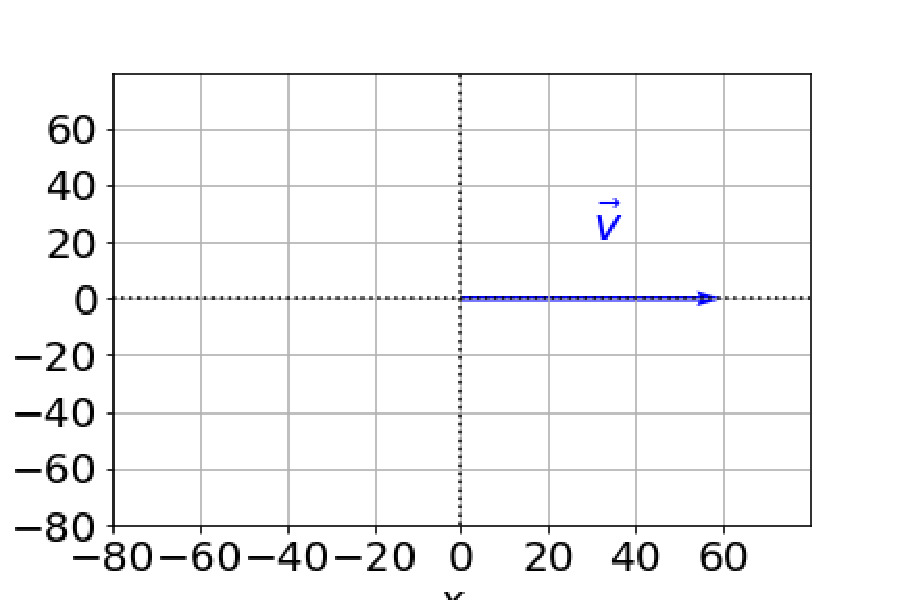
\includegraphics[height=.3\textheight]{images/fig-east.pdf}
                \[
                    \vec{v} = \vecOld{v} = \begin{bmatrix}
                        60 \\ 0
                    \end{bmatrix}
                \]
                \column{.33\textwidth}
                A car traveling $40$ miles per hour directly South.
                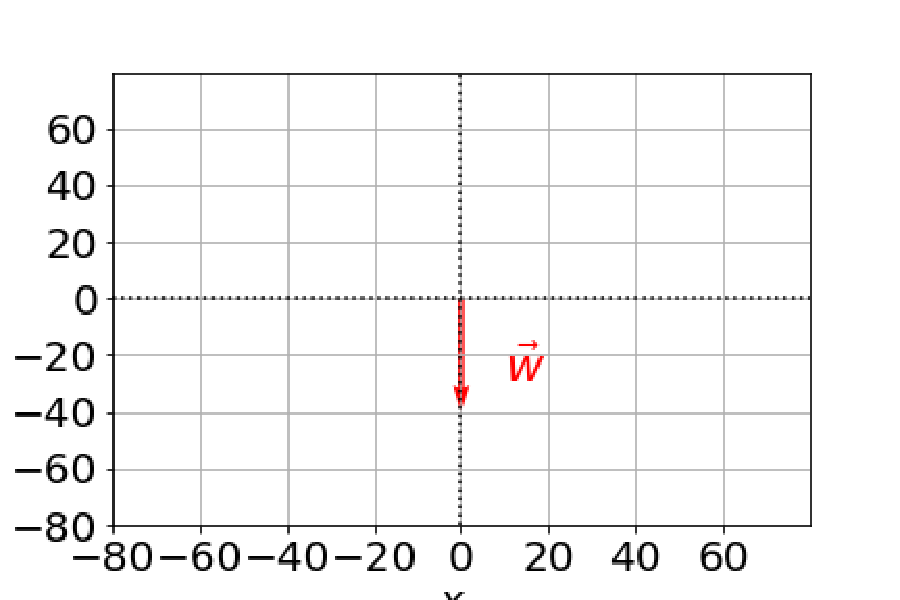
\includegraphics[height=.3\textheight]{images/fig-south.pdf}
                \[
                    \vec{w} = \vecOld{w}  = \begin{bmatrix}
                        0 \\ -40
                    \end{bmatrix}
                \]
                \column{.33\textwidth}
                A car traveling $64$ miles per hour directly North West.
                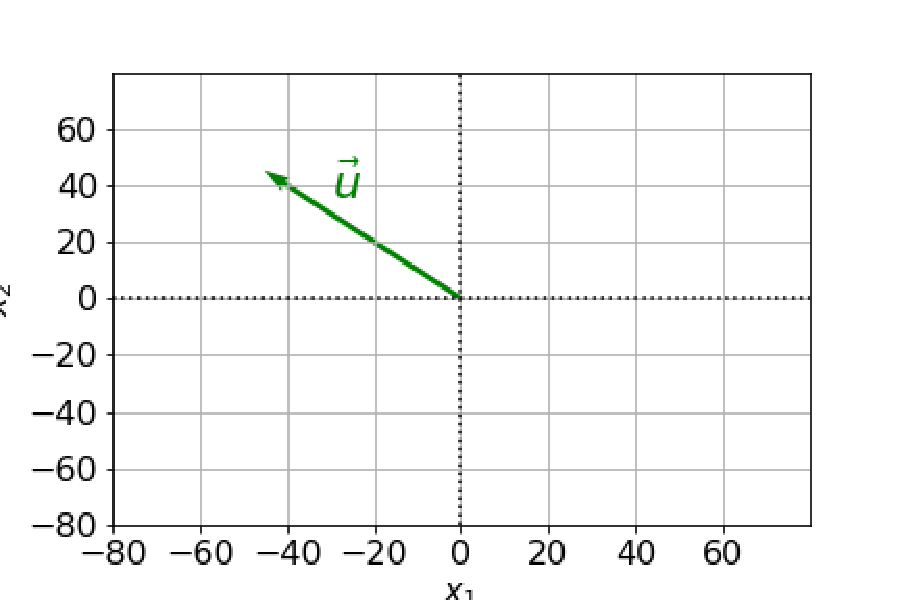
\includegraphics[height=.3\textheight]{images/fig-northwest.pdf}
                \[
                    \vec{u} = \vecOld{u} = \begin{bmatrix}
                        -\frac{64}{\sqrt{2}} \\ \frac{64}{\sqrt{2}}
                    \end{bmatrix}
                \]
            \end{columns}
        \end{example}
    \end{frame}
    \begin{frame}{Vectors in $\R^n$}
        \begin{defn}
            A \rText{column vector} (which we will from now on refer to as a vector) is a matrix with
            only $1$ column. \pause We denote vectors by:
            \begin{itemize}
                \item a lowercase bold letter like $\mathbf{v}$ or
                \item using an arrow above a lowercase letter like $\vecOld{v}$
            \end{itemize}
        \end{defn}
        \pause
        If the vector $\vec{v}$ has $n$ different real numbers, then we say that $\vec{v}\in\R^n$, and
        \[
            \vec{v} = \begin{bmatrix}
                v_1\\
                v_2\\
                \vdots\\
                v_n
            \end{bmatrix}
        \]
    \end{frame}
    \begin{frame}{Vector Equality}
        \begin{defn}
            \rText{Vector Equality}. We say that two vectors,
            $\vec{v} = \begin{bmatrix}v_1\\\vdots\\v_n\end{bmatrix}$
            $\vec{w} = \begin{bmatrix}w_1\\\vdots\\w_n\end{bmatrix}$ are \rText{equal} if and only if
                \pause
                \begin{itemize}
                    \item They have the \bText{same direction and length} or
                        \pause
                    \item All entries of the two vectors are the same:
                        \[
                            \bText{v_k = w_k\text{ for all }1\leq k\leq n}
                        \]
                \end{itemize}
        \end{defn}
    \end{frame}
    \begin{frame}{Vector Arithmetic (Addition)}
        \small
        \begin{defn}
            We define adding two vectors $\vec{u},\vec{v}\in\R^n$ as
            $
                \vec{u} + \vec{v} = \begin{bmatrix}
                    u_1 + v_1 \\
                    \vdots \\
                    u_n + v_n
                \end{bmatrix}.
            $ Note: This means that we can only add vectors with the same dimensions together! And the result will have the same dimension!
        \end{defn}
        \pause
        \begin{example}
            Adding the following vectors
            \begin{columns}
                \scriptsize
                \column{.5\textwidth}
                    $\vec{u} = \begin{bmatrix}1\\2\end{bmatrix}, \vec{v} = \begin{bmatrix}4\\1\end{bmatrix}$
                        \onslide<3->
                        \[
                            \vec{u}+\vec{v} = \begin{bmatrix}
                                1+4 \\
                                2+1
                            \end{bmatrix} = \begin{bmatrix}
                                5\\3
                            \end{bmatrix}
                        \]
                        \onslide<2->
                \column{.5\textwidth}
                    $\vec{u} = \begin{bmatrix}0\\-1\\5\end{bmatrix}, \vec{v} = \begin{bmatrix}7\\-5\\10\end{bmatrix}$
                        \onslide<3->
                        \[
                            \vec{u}+\vec{v} = \begin{bmatrix}
                                0+7 \\
                                -1 + -5\\
                                5 + 10
                            \end{bmatrix} = \begin{bmatrix}
                                7\\-6\\15
                            \end{bmatrix}
                        \]
                        \onslide<2->
            \end{columns}
        \end{example}
    \end{frame}
    \begin{frame}{Vector Arithmetic (Scalar Multiplication)}
        \scriptsize
        \begin{defn}
            A \rText{scalar} is a quantity with only magnitude and no direction. Think about numbers like $2,\sqrt{5},\pi,$etc.
        \end{defn}
        \pause
        \begin{defn}
            \rText{Scalar Product}: For a vector $\vec{v}\in\R^n$, and a scalar $c\in\R$. We define the \bText{scalar product} as $c\vec{v} = \begin{bmatrix}
                c\cdot v_1\\
                \vdots\\
                c\cdot v_n
            \end{bmatrix}
            $
            \pause

            Note: This means that we can multiply any scalar by any vector, and the dimension of the output is the same as the vector input
        \end{defn}
        \pause
        \begin{example}
            Computing the scalar product of the following

                $c=-3, \vec{v} = \begin{bmatrix}
                    2\\-5
                \end{bmatrix},$
                \onslide<5->\qquad\qquad\qquad\qquad\qquad
                $
                c\vec{v} = \begin{bmatrix}
                    -3\cdot 2\\-3\cdot -5
                \end{bmatrix} = 
                \begin{bmatrix}
                    -6\\15
                \end{bmatrix}
                $
                \onslide<4->
        \end{example}

\end{frame}
    \begin{frame}{Geometric Descriptions of Vectors in $\R^2$}
        \scriptsize
  

        {\small  We can think of the vector $\vec{v} = \begin{bmatrix} 
        v_1 \\ v_2 \end{bmatrix} \in \R^2$ as a directed line segment (an arrow).}

  \begin{columns}
    
 \column{0.5\textwidth}
 {\small Consider two vectors $\vec{u}$ and $\vec{v} \in \R^2$. The sum $\vec{u} + \vec{v}$ is  the result of first moving $\vec{u}$ and then moving $\vec{v}$.}

 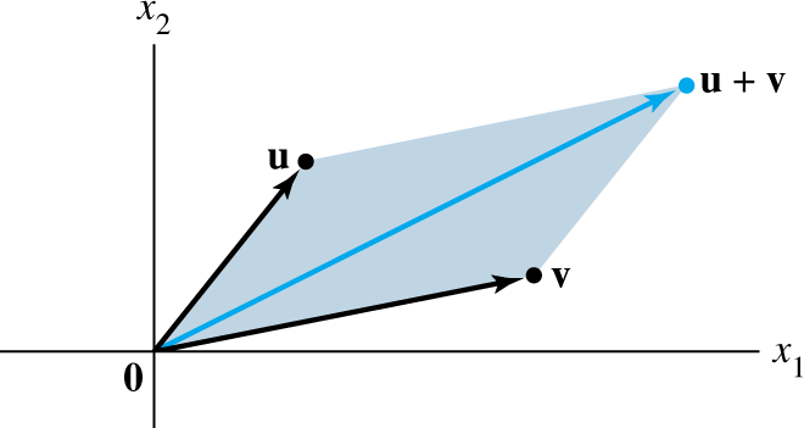
\includegraphics[width=0.9\tw]{images/fig-add.png}

 \column{0.5\tw}

 {\small Consider the vector $\vec{u} \in \R^2$ and nonzero scalar $c$. The scalar product $c \vec{u}$ gives a vector parallel to $\vec{u}$ whose magnitude has been scaled by a factor of $c$.
      \begin{itemize}
 \item If $c > 0$,  then $c \vec{u}$ has the same direction as $\vec{u}$.
 \item If $c < 0$,  then $c \vec{u}$ has the opposite direction as $\vec{u}$.
\item If $|c| < 1$, then $c \vec{u}$ is a compression of $\vec{u}$.
\item If $|c| > 1$, then $c \vec{u}$ is a stretching of $\vec{u}$.
      \end{itemize} }

  \end{columns}
        \begin{tcolorbox}
{\small  \rText{Parallelogram Rule for Addition}: If $\vec{u}$ and $\vec{v}$ are in $\R^2$, then the sum $\vec{u+v}$ is the diagonal of the parallelogram spanned by $\vec{u}$ and $\vec{v}$. }
        \end{tcolorbox}
    \end{frame}
\begin{frame}{Properties of Vector Arithmetic}
    \small
    \begin{tcolorbox}
        The \rText{zero vector} is defined as the vector in $\R^n$ with no magnitude, and it is denoted by $\vec{0}$ or $\vecOld{0}$. As a result of this definition, it follows that $\displaystyle \vec{0} = \begin{bmatrix} 0 \\ 0 \\ \vdots \\ 0 \end{bmatrix}$.
    \end{tcolorbox}

  For all $\vec{u}, \vec{v}, \vec{w}$ in $\R^n$ and all scalars $c$ and $d$:

  \begin{columns}[T]
    \column{0.5\textwidth}
    \begin{enumerate}[(i)]
      \item $\vec{u} + \vec{v} = \vec{v} + \vec{u}$
      \item $(\vec{u} + \vec{v}) + \vec{w} = \vec{u} + (\vec{v} + \vec{w})$
      \item $\vec{u} + \vec{0} = \vec{0} + \vec{u} = \vec{u}$
      \item $\vec{u} + (-\vec{u}) = \vec{0}$
      \end{enumerate}

    \column{0.5\textwidth}
      \begin{enumerate}[(i)]
    \setcounter{enumi}{4}
    \item $c(\vec{u}+\vec{v}) = c\vec{u}+c\vec{v}$
    \item $(c+d) \vec{u} = c\vec{u} + d \vec{u}$
    \item $c(d \vec{u}) = (cd) \vec{u}$
    \item $1 \vec{u} = \vec{u}$
      \end{enumerate}
  \end{columns}

  \end{frame}
    \begin{frame}{Linear Combinations of Vectors}
        \begin{defn}
            \rText{Linear Combination}: A \bText{linear combination} of vectors $\vec{v}_1,\dots,\vec{v}_p\in\R^n$ with 
            \bText{weights} $c_1,\dots,c_p\in\R$ is the vector $\vec{y}$ given by
            \[
                \vec{y} = c_1\vec{v}_1 + \cdots + c_p\vec{v}_p = \sum_{k=1}^p c_k\vec{v}_k
            \]
        \end{defn}
        \pause
        \begin{example}
            \[
                2\begin{bmatrix}
                    2\\1
                \end{bmatrix} + -3\begin{bmatrix} 
                    -1\\1
                \end{bmatrix}\pause = \begin{bmatrix}
                    2\cdot 2\\2\cdot 1
                \end{bmatrix} + \begin{bmatrix}
                    -3\cdot -1\\ -3\cdot 1
                \end{bmatrix}\pause =
                \begin{bmatrix}
                    4+3\\2-3
                \end{bmatrix}\pause =
                \begin{bmatrix}
                    7\\-1
                \end{bmatrix}
            \]
        \end{example}
    \end{frame}
    \begin{frame}{Giving Directions in a Grid}
        \begin{columns}
            \column{.5\textwidth}
            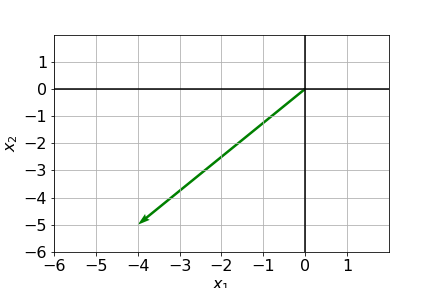
\includegraphics[width=.6\textwidth]{images/fig-span1.png}
            \column{.5\textwidth}
            \begin{example}
                Find constants $x_1$ and $x_2$ such that
                \[
                    \begin{bmatrix}
                        -4\\-5
                    \end{bmatrix} = x_1\begin{bmatrix}
                        1\\0
                    \end{bmatrix} + x_2\begin{bmatrix}
                        0\\1
                    \end{bmatrix}
                \]
            \end{example}
        \end{columns}
        \pause
        \begin{tcolorbox}
            The vectors $e_1 = \begin{bmatrix}
                1\\0
            \end{bmatrix}$ and $e_2 = \begin{bmatrix}
                0\\1
            \end{bmatrix}$ are the \rText{standard column vectors}.
        \end{tcolorbox}
    \end{frame}
    \begin{frame}{Giving Directions in a Different System}
        \begin{columns}
            \column{.7\textwidth}
            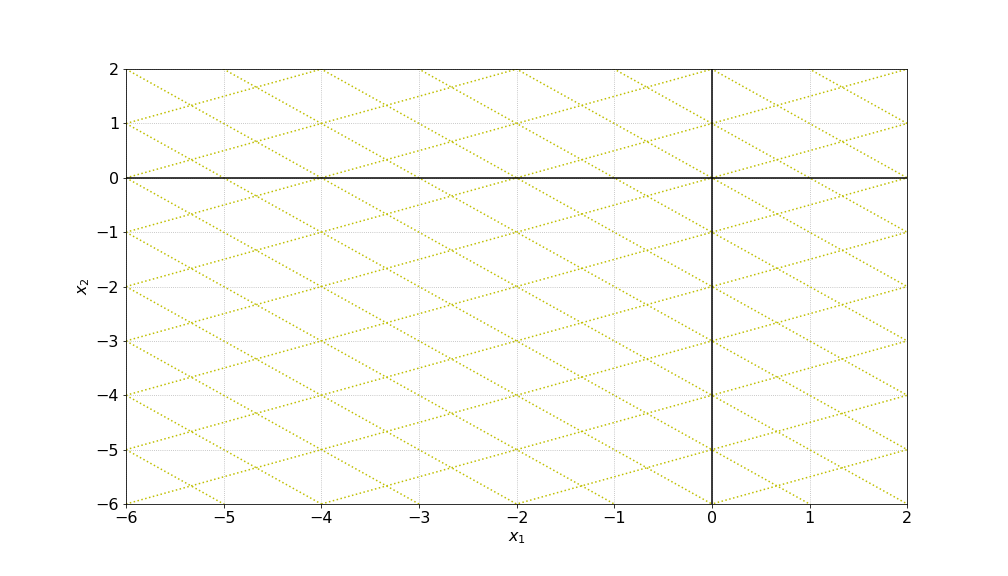
\includegraphics[width=\textwidth]{images/fig-span2.png}
            \column{.3\textwidth}
            \begin{example}
                Find constants $x_1$ and $x_2$ such that
                \[
                    \begin{bmatrix}
                        -4\\-5
                    \end{bmatrix} = x_1\begin{bmatrix}
                        2\\1
                    \end{bmatrix} + x_2\begin{bmatrix}
                        -1\\1
                    \end{bmatrix}
                \]
            \end{example}
        \end{columns}
    \end{frame}
    \begin{frame}{Solving for the Weights}
        \small
        First, let's simplify our statement!
        \[
            \begin{bmatrix}
                -4\\-5
            \end{bmatrix} = x_1\begin{bmatrix}
                2\\1
            \end{bmatrix} + x_2\begin{bmatrix}
                -1\\1
            \end{bmatrix} = \begin{bmatrix}
                2x_1 - x_2\\
                x_1 + x_2
            \end{bmatrix}
        \]
        \pause
        Which becomes
        \begin{align*}
            -4 &= 2x_1 - 1x_2\\
            -5 &= 1x_1 + 1x_2
        \end{align*}
        \pause
        Gaussian Elimination can solve this!
        \[
            \aMat{cc|c}{
                2 & -1 & -4\\
                1 & 1 & -5
            }\rightarrow\aMat{cc|c}{
                1 & 0 & -3\\
                0 & 1 & -2
            }
        \]
        So, $(x_1,x_2) = (-3,-2)$. Or we can say
        $
            \vec{x} = \begin{bmatrix}
                -3\\-2
            \end{bmatrix}
        $
    \end{frame}
    \begin{frame}{What Our Directions Look Like}
        \begin{columns}
            \column{.7\textwidth}
            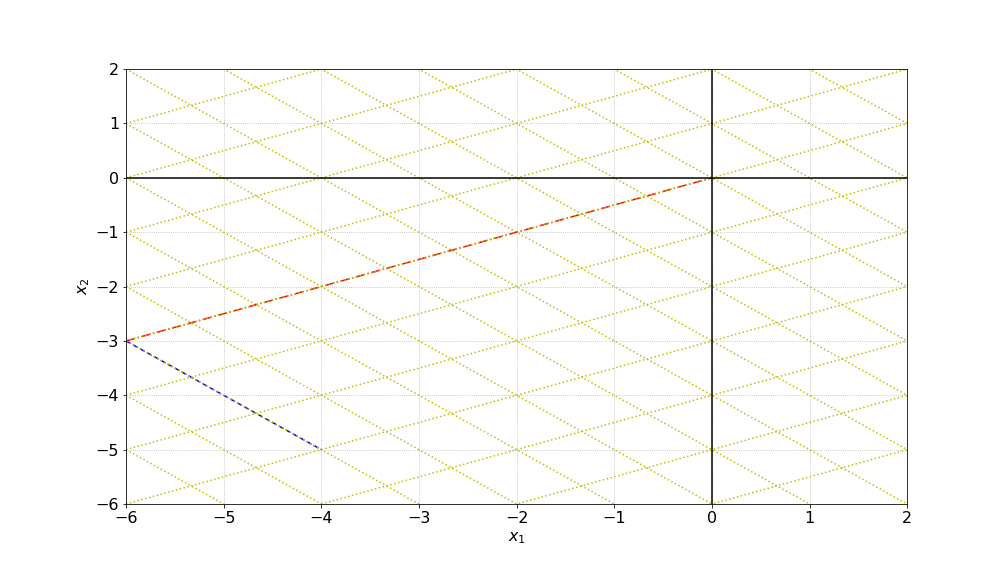
\includegraphics[width=.8\textwidth]{images/fig-span3.png}
            \column{.3\textwidth}
            \[
                \vec{x} = \begin{bmatrix}
                    \rText{-3}\\\bText{-2}
                \end{bmatrix}
            \]
        \end{columns}
        \pause
        What about an arbitrary vector $\vec{w}\in\R^2$?\pause\  Can we find an $\vec{x}$ such that
        \[
            \begin{bmatrix}
                w_1\\w_2
            \end{bmatrix} = x_1\begin{bmatrix}
                2\\1
            \end{bmatrix} + x_2\begin{bmatrix}
                -1\\1
            \end{bmatrix}
        \]

    \end{frame}
    \begin{frame}{Span of a Set of Vectors}
        \begin{defn}
            \rText{Span}: Let $\vec{v}_1,\dots,\vec{v}_p\in\R^n$. 
            Then we define $\bText{\Span{\vec{v}_1,\dots,\vec{v}_p}}$ 
            to be the subset of $\R^n$ containing all linear combinations 
            of $\vec{v}_1,\dots,\vec{v}_p$.\pause\ In other words
            \[
                \Span{\vec{v}_1,\dots,\vec{v}_p} = \set{\vec{y}\in\R^n}
                {\vec{y} = \sum_{k=1}^pc_k\vec{v}_k\text{ for some }
                c_1,\dots,c_p\in\R}
            \]
        \end{defn}
        \pause
        How do we test if $\vec{y}\in\Span{\vec{v}_1,\dots,\vec{v}_p}$?
        \pause
        \begin{solution}
            Solve the system \[
                \aMat{ccc|c}{
                    \vec{v}_1 & \cdots & \vec{v}_p & \vec{y}
                }
            \]
        \end{solution}
    \end{frame}
    \begin{frame}{Span Example}
        \small
        \begin{example}
            Describe the span of the vectors $\vec{v}_1,\vec{v}_2$ given by
            \[
                \vec{v}_1 = \begin{bmatrix}
                    1\\0\\1
                \end{bmatrix}
                \qquad
                \vec{v}_2 = \begin{bmatrix}
                    0\\2\\1
                \end{bmatrix}
            \]
            \pause
            \begin{solution}
                \scriptsize
                \[
                    c_1\vec{v}_1 + c_2\vec{v}_2 = c_1\begin{bmatrix}
                        1\\0\\1
                    \end{bmatrix} + c_2\begin{bmatrix}
                        0\\2\\1
                    \end{bmatrix} = \begin{bmatrix}
                        c_1 \\ 2c_2\\ c_1 + c_2
                    \end{bmatrix}
                \]
                So,
                \[
                    \Span{\vec{v}_1,\vec{v}_2} = \set{\vec{y}\in\R^3}
                    {\vec{y} = \begin{bmatrix}
                        c_1\\2c_2\\c_1+c_2
                    \end{bmatrix}\text{ for some }c_1,c_2\in\R}
                \]
            \end{solution}
        \end{example}
    \end{frame}
    \begin{frame}{Span of a Set of Vectors Practice}
        Describe the span of the following vectors
        \vfill
        \begin{columns}
            \column{.5\textwidth}
            \begin{enumerate}
                \item $\vec{v}_1 = \begin{bmatrix}
                        0\\1\\1
                \end{bmatrix}$
                \vspace{35pt}
                \item $\vec{v}_1 = \begin{bmatrix}
                        2\\1
                \end{bmatrix}, \vec{v}_2 = \begin{bmatrix}
                    -4\\-2
                \end{bmatrix}$
            \end{enumerate}
            \column{.5\textwidth}
            \begin{enumerate}
                    \addtocounter{enumi}{2}
                \item $\vec{v}_1 = \begin{bmatrix}0\\0\end{bmatrix}$
                \vspace{35pt}
                \item $\vec{v}_1 = \begin{bmatrix}1\\0\\-2\end{bmatrix},
                        \vec{v}_2 = \begin{bmatrix}0\\1\\-1\end{bmatrix}$
            \end{enumerate}
        \end{columns}
    \end{frame}
    \iftoggle{showSolutions}{
    \begin{frame}{Span of a Set of Vectors Practice Solutions}
        \small
        Describe the span of the following vectors
        \vfill
        \begin{columns}
            \column{.5\textwidth}
            \begin{enumerate}
                \item $\vec{v}_1 = \begin{bmatrix}
                        0\\1\\1
                \end{bmatrix}$.

                    {\scriptsize $
                        \Span{\vec{v}_1} = \set{\vec{y}\in\R^3}
                        {\vec{y}=\begin{bmatrix}0\\c_1\\c_1
                        \end{bmatrix}\text{ for some }c_1\in\R}
                    $}
                \item $\vec{v}_1 = \begin{bmatrix}
                        2\\1
                \end{bmatrix}, \vec{v}_2 = \begin{bmatrix}
                    -4\\-2
                \end{bmatrix}$

                    {\scriptsize $
                        \Span{\vec{v}_1,\vec{v}_2} = \set{\vec{y}\in\R^2}
                        {\vec{y}=\begin{bmatrix}2c_1 - 4c_2\\c_1-2c_2
                        \end{bmatrix}\text{ for some }c_1,c_2\in\R}
                    $}
            \end{enumerate}
            \column{.5\textwidth}
            \begin{enumerate}
                    \addtocounter{enumi}{2}
                \item $\vec{v}_1 = \begin{bmatrix}0\\0\end{bmatrix}$

                    {\scriptsize $
                        \Span{\vec{v}_1} = \setBasic{\begin{bmatrix}0\\0\end{bmatrix}}
                    $}
                \item $\vec{v}_1 = \begin{bmatrix}1\\0\\-2\end{bmatrix},
                        \vec{v}_2 = \begin{bmatrix}0\\1\\-1\end{bmatrix}$

                    {\scriptsize $
                        \Span{\vec{v}_1,\vec{v}_2} = \set{\vec{y}\in\R^3}
                        {\vec{y}=\begin{bmatrix}c_1\\c_2\\-2c_1-c_2
                        \end{bmatrix}\text{ for some }c_1,c_2\in\R}
                    $}
            \end{enumerate}
        \end{columns}
    \end{frame}
    }{}
    \begin{frame}{More Span Practice}
        \centering
        Determine if $y=
            \begin{bmatrix}
                4\\5\\-1
            \end{bmatrix}$
 is in $\Span{\begin{bmatrix}1\\0\\-2\end{bmatrix},
            \begin{bmatrix}0\\1\\-1\end{bmatrix}}$
                \iftoggle{showSolutions}{

                    \vspace{20pt}\pause
                    Perform Gaussian Elimination on the augmented matrix\pause
                    \[
                        \aMat{cc|c}{
                            1 & 0 & 4\\
                            0 & 1 & 5\\
                            -2&-1 &-1
                        }\pause\rightarrow\aMat{cc|c}{
                            1 & 0 & 4\\
                            0 & 1 & 5\\
                            0 & 0 & 12
                        }
                    \]
                    \pause
                    No!
                }{\vspace{150pt}}
    \end{frame}
    \begin{frame}{Systems with Infinite Solutions}
        \small
        Recall for the system,
        \begin{align*}
            1x_1 + 2x_2 + x_3 &= -2\\
            1x_1 + 3x_2 - 2x_3&= 1
        \end{align*}
        Our answer is
        \pause
        \[
            \begin{cases}
                x_1 &= -8-7x_3\\
                x_2 &= 3+3x_3\\
                x_3 &\text{is free}
            \end{cases}
        \]
        \pause
        But writing this can be cumbersome!
    \end{frame}
    \begin{frame}{Using Vectors!}
        We recall from earlier that we can write out our answer in terms of vectors!
        \[
            \vec{x} = \begin{bmatrix}
                -8-7x_3\\
                3+3x_3\\
                x_3
            \end{bmatrix}\pause = \begin{bmatrix}
                -8\\
                3 \\
                0
            \end{bmatrix} + \begin{bmatrix}
                -7x_3\\
                3x_3\\
                x_3
            \end{bmatrix}\pause = \begin{bmatrix}
                -8\\
                3 \\
                0
            \end{bmatrix} + x_3\begin{bmatrix}
                -7\\
                3\\
                1
            \end{bmatrix}
        \]
        \pause
        But what is $x_3$?\pause It's just some real number, so we can use any letter we want. Let's use $s$.
        \pause
        \[
            \vec{x} = \begin{bmatrix}
                -8\\3\\0
            \end{bmatrix} + s\begin{bmatrix}
                -7\\3\\1
            \end{bmatrix}
        \]
    \end{frame}
    \begin{frame}{Span of a Set of Vectors Conceptual Practice}
        Let $\vec{v}_1,\vec{v}_2,\vec{v}_3,\vec{w}$ be vectors in $\R^n$. 
        Prove that if $\vec{w}\in\Span{\vec{v}_1,\vec{v}_2,\vec{v}_3}$, then

        $\Span{\vec{v}_1,\vec{v}_2,\vec{v}_3,\vec{w}} = \Span{\vec{v}_1,\vec{v}_2,\vec{v}_3}$
        \vspace{150pt}
    \end{frame}
\end{document}
